\subsection*{Background}
\textbf{Morse homology}. The field of differential topology studies the connection between analysis on a smooth $n$-manifold $M$ and its underlying topology. This field was pioneered by Morse in the beginning of the 20th century, and further developed by Smale, Thom, Milnor and more. A key idea in this theory is handle decomposition (Smale \cite{smale1962structure}) which goes as follows. Given a ``nice'' (namely, Smale and Morse) function $f \colon M\to R$, we can decompose $M$ as follows: for each critical point, we glue a copy of $H^j = D^j \times D^{n-j}$ (a $j$-handle), where $j$ is the signature of the Hessian of the critical point (the \textbf{index}). By retracting $H^j$ to $D^j$, we obtain a CW structure on $\Man$.

Once we have a CW structure, we can attempt to read off algebraic-topological invariants of $\Man$. The data of the number and dimensions of the cells, given by the number of critical points and their indices, can recover the Euler characteristic.

To gain a deeper understanding of the topology of the manifold, we analyze the attaching maps of the handles corresponding to critical points. A key tool in this analysis is the \textbf{moduli space of flow lines}. Given a Smale-Morse function $ f: M \to \bbR $, let $ y $ and $ x $ be critical points of $ f $. A \textbf{flow line} from $ y $ to $ x $ is a path $ \gamma: \bbR \to M $ satisfying the differential equation:
\begin{equation*}
\frac{d\gamma}{dt} + \nabla_\gamma f = 0,
\end{equation*}
with boundary conditions $ \gamma(-\infty) = y $ and $ \gamma(\infty) = x $. We define the \textbf{moduli space of flow lines} from $ y $ to $ x $, denoted by $ \flowM(z,x) $, as the set of such flow lines modulo reparametrization by time translation. Under generic conditions, $ \flowM(y, x) $ is a smooth (not necessarily closed) manifold of dimension $ \Ind(y) - \Ind(x) - 1 $.

To define the \textbf{Morse chain complex}, let $ C_p $ be the free abelian group generated by the critical points of index $ p $:
\begin{equation*}
C_p = \bigoplus_{\Ind(x) = p} \mathbb{Z} \langle x \rangle.
\end{equation*}
For critical points $ y $ and $ x $ with $ \Ind(y) = \Ind(x) + 1 $, the moduli space $ \flowM(y, x) $ is a compact, zero-dimensional manifold. By assigning an orientation to each flow line, in a compatible way, we can count the signed number of points in $ \flowM(y, x) $. The \textbf{differential} $ d: C_p \to C_{p-1} $ is then defined by:
\begin{equation*}
d(y) = \sum_{\Ind(x) = \Ind(y) - 1} \# \flowM(y, x) \cdot x,
\end{equation*}
where $ \# \flowM(y, x) $ denotes the signed count of flow lines from $ y $ to $ x $. Later, we will see that $ d^2 = 0 $, which follows from the structure of the compactified moduli spaces $ \overline{\flowM(z, x)} $ and their boundaries.

The resulting chain complex $ (C_*, d) $ is quasi-isomorphic to the cellular chain complex of $ M $, and its homology, called \textbf{Morse homology}, computes the singular homology of $ M $. This allows us to distinguish manifolds like $ \mathbb{RP}^3 $ and $ S^1 \times S^2 $, though more refined tools are needed to distinguish $ \mathbb{CP}^2 \# \mathbb{CP}^2 $ and $ S^2 \times S^2 $.

\textbf{Flow Manifolds and Higher Gluing Maps}. An important result in differential topology is the \textbf{Pontryagin-Thom isomorphism}. Given a smooth manifold $\Man$, a normal \textbf{framing} of a closed submanifold $\Sigma \subseteq \Man$ with codimension $k$, is choice of a trivialization of the normal bundle $\nu \Sigma \simeq \Sigma\times \bbR^k$. A closed submanifold with a framing is called \textbf{framed manifold}. Two normally framed submanifolds $\Sigma_1, \Sigma_2$ are \textbf{cobordant} if there is a normally framed submanifold with boundary $W \subseteq [0,1] \times M$ with $\partial W = \Sigma_1 \sqcup \Sigma_2$ in a way that compatible with the framing. The work of Pontryagin and Thom shows an isomorphism between $k$-dimensional normally framed submanifolds of $\Man$ up to cobordism and the $(n-k)$th cohomotopy group of $\Man$ (maps $\Man \to S^{n-k}$ up to homotopy), which we denote by:
\begin{equation*}
    \Omega^{\fr}_k(\Man) \overset{PT}{\simeq} [\Man,S^{n-k}].
\end{equation*}
The map from the RHS is given by sending a map $\Man \to S^n$ to the preimage $f^{-1}(r)$ of a regular value.
We remind that given a CW complex $Y$ and two successive cells with dimensions $j$ and $i$ (such that there are no cells with dimensions between $j$ and $i$), the attaching map between them is a map $\partial D^j \to (D^i)_+$ which is represented as a class in $[S^{j-1},S^i]$. Using the Pontryagin isomorphism, we obtain a $j-i-1$ dimensional normally framed submanifold of $S^{j-1}$.

Given a Smale-Morse function on a smooth manifold $f:\Man \to \bbR$ and two critical points $z, x$, we denote by $\flowM(z,x)$ the moduli space of flow lines from $z$ to $x$ and call it the \textbf{flow manifold}. Generally, these manifolds are open, and we compactify them. The boundary of the compactified manifolds is given by flowing from $z$ to $x$ through a critical point $y$:
\begin{equation*}
    \partial \overline{\flowM(z,x)} = \bigcup_{\Ind(z) > \Ind(y) > \Ind(x)} \overline{\flowM(z,y)} \times \overline{\flowM(y,x)},
\end{equation*}
which gives the (compactified) flow manifold the structure of a \textbf{manifold with corners}. We can ask what these manifolds tell us about the homotopy of $\Man$.

Franks, in \cite{franks1979morse}, showed that if $f:\Man \to \bbR$ is a Morse-Smale function on a smooth manifold and $q,p$ are successive critical points (there are no critical points with index between $q$ and $p$), then the moduli space of flow lines from $q$ to $p$ is a $(\Ind(p)-\Ind(q)-1)$ normally framed submanifold of $S^{\Ind(q)-1}$, which corresponds under Pontryagin-Thom isomorphism to the attaching map between $q$ and $p$. We can use this result to distinguish between $\mathbb{CP}^2 \# \mathbb{CP}^2$ and $S^2 \times S^2$. The first has a non-trivial framing on the manifold between the maximum and each of the middle points, while the second has a trivial framing on the flow manifolds.

\textbf{Generalized homology}. Instead of considering homology over $\bbZ$, we can consider generalized homology over a spectrum. Given a manifold $\Man$ and a generalized homology theory $F$ (which we think of as a spectrum), we can ask whether there is a way to calculate $F_*(\Man)$ using the geometric data of a Morse function on $\Man$.

To do so, one can ask what the generalization of calculating homology using the cellular structure of a CW complex is. The answer is the \textbf{Atiyah-Hirzebruch spectral sequence}, a homological bookkeeping mechanism that calculates generalized homology of a CW complex.

This idea goes back to Floer. In \cite{floer1989witten}, he conjectured that it should be possible to obtain $F_*(\Man)$ in a way similar to Morse homology through an analysis of trajectory spaces (flow manifolds). In particular, he suggested that a reasonable modification of the ideas above should lead to a spectral sequence converging to (co)homology with coefficients in $\mathbb{S}$ - the spectrum representing stable homotopy.

A related question is the analysis of real-valued functions on objects that are not finite-dimensional closed manifolds. Floer developed this idea in the 1980s, which led to Floer theory. This field has two main flavors: symplectic and low-dimensional. Symplectic Floer theory studies action functionals on the (infinite-dimensional) space of loops in a manifold or on the space of paths between two submanifolds. In low-dimensional topology, the ideas of Morse theory are generalized to study manifolds by analyzing a functional on a space of connections on a bundle over a 3-manifold. 

In both of these branches, we ultimately obtain a chain complex, and hence a homology group. One can ask whether these homology groups are actually the (cellular) homology groups of some space. Are Floer homology groups the shadow of a more structured object?

The development of the framework to answer these questions led CJS (Cohen, Jones, and Segal) in \cite{CJS95} to introduce \textbf{framed flow categories}, which axiomatize the data extracted from a Smale-Morse function on a manifold. In short, a framed flow category $\fC_f$ is a set of objects (correspond to critical points) with a grading function $\norm{-}$ (correspond to the index). For two objects $b,a$, the morphism space between $b$ and $a$ is an $\norm{b}-\norm{a}-1$ dimensional manifold with corners $M_{b,a}$ with a choice of trivialization $TM_{b,a} \oplus \underline{\bbR^k}$ for some $k$ (correspond to the framed flow manifold).
Moreover, the faces of the boundary $\partial \flowM_{c,a}$ are given by the images of the composition
\begin{equation*}
    \flowM_{c,b} \times \flowM_{b,a} \hookrightarrow \flowM_{c,a}
\end{equation*}

\textbf{Coherent chain complexes and filtered objects.} Given a \textbf{filtered space} $F_0 \to \dots \to F_n = F$, for example by taking a CW complex with the skeletal filtration, we can take the quotients $F_p/F_{p-1}$ and obtain maps $\partial_{p}:F_{p}/F_{p-1} \to \Sigma F_{p-1}/F_{p-2}$, which combine into a sequence of spaces $\{K_p\}$ given by
\begin{equation*}
    F_n/F_{n-1} \to \Sigma F_{n-1}/F_{n-2} \to \dots \to \Sigma^{n} F_0
\end{equation*}
with the property that $\partial_{p+1} \circ \partial_p$ is null-homotopic. Taking homology with $\mathbb{Z}$ coefficients gives the cellular chain complex of $F$. The fact that $\Ab$ is a 1-category implies that there are no higher morphisms in the cellular chain complex. However, the chain $K$ viewed as a chain in the $\infty$-category of homotopy types/spectra has higher morphisms. $F$ always comes with canonical null-homotopies of $\partial_{p+1} \circ \partial_p$. Moreover, any 3-composition
\begin{equation*}
    F_{n+3}/F_{n+2} \to \Sigma F_{n+2}/F_{n+1} \to \Sigma^2 F_{n+1}/F_{n} \to \Sigma^3 F_{n}/F_{n-1}
\end{equation*}
admits two null-homotopies, which are two paths $I \to \Map(F_{n+3}/F_{n+2}, \Sigma^3 F_{n}/F_{n-1})$ that agree on $\{0\}\times A$ and $ \{1\}\times A$. Hence, we can concatenate them to a map $S^1 \to \Map(F_{n+3}/F_{n+2}, \Sigma^3 F_{n}/F_{n-1})$. Part of the data of $K$ is a null-homotopy of this loop. We call the sequence $\{K_p\}$ with all the higher coherences a \textbf{coherent chain complex}.

We can try to recover the filtered object $F$ from the chain $K$. For example, given a filtered pointed space:
\begin{equation*}
    F_0 \to F_1 \to F_2
\end{equation*}
we get a chain complex:
\begin{equation*}
    K_2 = F_2/F_1 \to \Sigma^1 F_1/F_0 \to \Sigma^2 F_0 = K_0.
\end{equation*}
By taking \textbf{iterated cofibers}, we can recover $F$ up to suspension:
\begin{equation*}
    \Sigma^2 F_0 = K_0, \quad \Sigma^2 F_1 = \cof \left (\Sigma^1 F_1/F_0 \to \Sigma^3 F_0\right ) = \cof (K_1 \to K_0 ),
\end{equation*}
and then we need to take iterated cofiber:
\begin{equation*}
    \Sigma^2 F_2 = \cof(\Sigma^1 F_2/F_0 \to \Sigma^2 F_0) = \cof \left ( \cof \left (F_2/F_1 \to \Sigma^1 F_1/F_0\right ) \to F_0 \right).
\end{equation*}
Hence, we can recover the stable homotopy type (spectrum) $\Sigma^\infty F_i$.

The idea of a coherent chain complex appeared in \cite{CJS95} and was organized using a topologically enriched model category. It is worth mentioning that in \cite{Ari21}, Ariotta and Krause used Lurie's modern framework of $\infty$-categories to give coherent chain complexes the structure of an $\infty$-category and showed an equivalence of categories between coherent chain complexes in spectra and (complete) filtered spectra. 
We denote the equivalence by 
\begin{equation*}
    \cA: \Fil(\cC) \simeq \Ch(\cC) : \cI
\end{equation*}

Briefly, CJS showed that a framed flow category $\fC$, can be collapsed (by Pontryagin Thom construction) to a coherent chain complex $K_{\fC} \in \Ch(\Sp)$ see \ref{constr:FF_to_Ch} for details. After taking iterated cofiber, we get a spectrum.
We define the \textbf{realization} of a framed flow category to be the\todo{ind?} spectrum
\begin{defn}\label{def:realofFFCat}
    \begin{equation}
        \norm{\fC} \coloneqq \colim \cI(K_{\fC})
    \end{equation}    
\end{defn}
\begin{rem*}
    Note that $\norm{\fC}$ depends on the choice of framing for the manifolds $M_{b,a}$.
\end{rem*}

To combining the ideas of framed flow categories and chain complexes: let $f: \Man \to \bbR$ be a manifold with a Smale-Morse function. First, we can construct from it a framed flow category $\fC_f$, then we collapse it to chain complex $\fC_f$ and realize it $\norm{\fC_f} \in \Sp$. A result by CJS states that
\begin{equation*}
    \norm{\fC_f} \simeq \Sinf \Man.
\end{equation*}

The fact that we can recover the stable homotopy type of $\Man$ from its framed flow category motivates the idea that we can read off a (generalized) homology of $\Man$ using the flow manifolds.

\subsection*{Notations}
We denote by $\Top$ the category of topological spaces, by $\Spaces$ the category of homotopy types/$\infty$-groupoids and $\Sp$ is the category of spectra, the stabilization functor is denoted $\Sinf: \Spaces \to \Sp$, and $\Ch(\Sp), \Fil(\Sp)$ are the categories of coherent chain complexes in Spectra and (complete) filtered Spectra.

For a topological space $Y$, we denote by $Y_+$ its one-point compactification (if $Y$ is compact, then $Y_+ = Y \cup \{*\}$).
For a CW complex $Y$, we denote by $\sk^k X$ its $k$-th skeleton.

For a stable tangential structure $\xi: \cX \to BO$, we denote by $\Omega^{\cX}_*$ the graded $\cX$-bordism ring and by $M\cX$ the Thom spectrum of $\cX$ structure.

In this paper, a manifold is assumed to be a \textbf{closed manifold} unless stated otherwise.

Let $\fC$ be a flow category, for $q,p \in \bbZ$ we denote the full subcategory on objects
\begin{equation*}
    \{x \in \ob(\fC), q \ge \norm{x}\ge p\}
\end{equation*}
by $\fC_{[q,p]}$, and $\fC_p \coloneqq \fC_{[p,p]}$. For brevity we denote
\begin{equation*}
    M_{p,q}\coloneqq \bigsqcup_{y \in \fC_q, x \in \fC_p} M_{y,x}.
\end{equation*}

Moreover, for a stable tangential structure $\xi: \cX \to BO$, we can define $\cX$ flow categories, as flow categories such that the morphism manifolds have $\cX$ structure which is compatible with the composition (instead of stable framing). For an $\cX$ flow category $\fC$, we get that $K_{\fC}$ is a coherent chain complex in $\Mod_{M\cX}$ and similarly to \cref{def:realofFFCat} we define $\norm{\fC} \in \Mod_{\cX}$ to be the colimit, but in $\Mod_{\cX}$.

\subsection*{Our results}
For a flow category $\fC$ with an $\cX$ tangential structure, we construct a spectral sequence where each page and differential reflect underlying geometric structures. This relationship provides a tool for analyzing the homotopy groups of the realization $\norm{\fC}$.

\begin{defn}\label{def:Xrnp-extension}
Let $\fC$ be a flow category, $n,p,r \in \bbN$ and let $X = {X_z} \in \bigoplus_{z \in \fC_p} \Omega^{\operatorname{\cX}}_{n - p}$, represented by disjoint union of manifolds.
An \textbf{$(X,r,n,p)$-extension} of $\fC$ is a flow category $\fC'$ with
\begin{equation*}
    \ob(\fC') = \fC_{[p,p-r]} \sqcup \{x\},\quad \norm{x}-p-1 = n-p
\end{equation*}
such that the flow manifold of $\fC'$, which denoted by $X_{a,b}$, satisfies:
\begin{equation*}
    X_{x, z} \simeq X_z,
\end{equation*}
and
\begin{equation*}
    X_{y,v} \simeq \flowM_{y,v}
\end{equation*}
for any $y,v \in \fC_{[p,p-r]}$.
\end{defn}
% surviev to r page iff r-1 extend
\begin{defn}\label{def:smallToda}
    Let $\fC'$ be a $(X,r,n,p)$-extension of $\fC$ and $y \in \fC_{p-(r+1)}$. We can define the punctured cube diagram:
    \begin{equation*}
        D_y: \ P(\{p,\dots,p-r\}) \setminus \varnothing \to \Top
    \end{equation*}
    where $P(-)$ is the power set, by
    \begin{equation*}
        D_y(\{a_1, \dots, a_k\}) = X_{x,a_1} \times M_{a_1,a_2} \dots \times M_{a_{k-1},a_k} \times M_{a_k,y}.
    \end{equation*}
    
    The \textbf{Toda manifold} is the colimit
    \begin{equation*}
        \colim D_y
    \end{equation*}
\end{defn}
We will see later that indeed, the Toda manifolds have a manifold structure and they are closed, $n-p+r$ dimensional, and $\cX$-structured.

\begin{exmp*}
    In \cref{fig:ffCat}, \ref{fig:test1}, \ref{fig:test2} we can see example of an extension and it's Toda manifold.
    \begin{center}
    % https://q.uiver.app/#q=WzAsNSxbMCwwLCJcXGJ1bGxldCJdLFswLDEsInhfMyJdLFswLDIsInhfMiJdLFswLDMsInhfMSJdLFswLDQsInhfMCJdLFswLDEsIk49IC0gXFwgLSIsMSx7ImxhYmVsX3Bvc2l0aW9uIjo4MCwic3R5bGUiOnsiYm9keSI6eyJuYW1lIjoibm9uZSJ9LCJoZWFkIjp7Im5hbWUiOiJub25lIn19fV0sWzEsMiwiTV97MywyfSA9ICtcXCArIiwxLHsic3R5bGUiOnsiYm9keSI6eyJuYW1lIjoibm9uZSJ9LCJoZWFkIjp7Im5hbWUiOiJub25lIn19fV0sWzIsMywiTV97MiwxfSA9ICtcXCAtIiwxLHsibGFiZWxfcG9zaXRpb24iOjIwLCJzdHlsZSI6eyJib2R5Ijp7Im5hbWUiOiJub25lIn0sImhlYWQiOnsibmFtZSI6Im5vbmUifX19XSxbMyw0LCJNX3sxLDB9ID0gKyIsMSx7ImxhYmVsX3Bvc2l0aW9uIjoyMCwic3R5bGUiOnsiYm9keSI6eyJuYW1lIjoibm9uZSJ9LCJoZWFkIjp7Im5hbWUiOiJub25lIn19fV0sWzIsNCwiSSIsMSx7ImN1cnZlIjotNX1dLFsxLDMsIkkgXFwgSSIsMSx7ImN1cnZlIjo0fV0sWzAsMiwiSSBcXCBJIiwxLHsiY3VydmUiOi01fV0sWzEsNCwiSV4yIiwxLHsiY3VydmUiOjUsImxldmVsIjoyfV0sWzAsMywiSV4yIiwxLHsiY3VydmUiOi01LCJsZXZlbCI6Mn1dXQ==
\begin{tikzcd}[column sep=huge]
    x & {x_4} & {x_3} & {x_2} & {x_1}
    \arrow["{X= - \sqcup -}"'{yshift=-5pt},curve={height=-10pt}, from=1-1, to=1-2, thick, dashed]
    \arrow["{X_{5,3}=I \sqcup I}"{description}, curve={height=30pt}, from=1-1, to=1-3, color=myred, dashed]
    %\arrow["{X_{5,2}=I^2}"{description}, curve={height=60pt}, Rightarrow, from=1-1, to=1-4, color=myblue, dashed]
    \arrow["{X_{5,2}=I^2}"{description}, curve={height=60pt}, from=1-1, to=1-4, color=myblue, dashed]
    \arrow["M_{4,2}={I \sqcup I}"'{description}, curve={height=-30pt}, from=1-2, to=1-4, color=mygreen]
    \arrow["M_{3,1}=I"{description}, curve={height=-30pt}, from=1-3, to=1-5, color=myyellow,crossing over]
    %\arrow["{M_{4,1}=I^2}"{description}, curve={height=-60pt}, Rightarrow, from=1-2, to=1-5, color=myviolet]
    \arrow["{M_{4,1}=I^2}"{description}, curve={height=-60pt}, from=1-2, to=1-5, color=myviolet]
    \arrow["{M_{4,3} = - \sqcup +}"'{yshift=-5pt},curve={height=-10pt}, from=1-2, to=1-3]
    \arrow["{M_{3,2} = + \sqcup -}"'{yshift=-5pt},curve={height=-10pt}, from=1-3, to=1-4]
    \arrow["{M_{2,1} = +}"'{yshift=-5pt},curve={height=-10pt}, from=1-4, to=1-5]
\end{tikzcd}
    \captionof{figure}{
    The solid part is the flow category $\fC$, it's objects are the $x_i$'s with $\norm{x_i}=i$, the arrows represent the morphism manifolds.
    The 0 dimensional manifold $X$ represent an element in $E_1^{4,4} = \Omega^{\fr}_{4-4}$.
    The dashed arrows are an $(X,2,4,4)$-extension.
    Notice that the whole diagram is not representing a flow category, $X_{5,1}$ is missing.
    The $\pm,I$ are the flow manifolds themselves (we omit the framing for clarity).
    }\label{fig:ffCat}
    \end{center}

    \captionsetup{font={small}}
    \begin{figure}
    \centering
    \begin{minipage}{.63\textwidth}
      \centering
      \adjustbox{width=\linewidth}{\begin{tikzcd}
{X\times M_{4,3}\times M_{3,2}\times M_{2,1}} && |[myyellow]|{X\times M_{4,3}\times M_{3,1}}& \\
\\
& |[mygreen]|{X\times M_{4,2}\times M_{2,1}} && |[myviolet]|{X\times M_{4,1}} \\
\\
|[myred]|{X_{5,3}\times M_{3,2}\times M_{2,1}} && |[orange]|{X_{5,3} \times M_{3,1}} \\
\\
& |[myblue]|{X_{5,2}\times M_{2,1}}
\arrow[gray,from=1-1, to=1-3]
\arrow[gray,from=1-1, to=3-2]
\arrow[gray,from=1-1, to=5-1]
\arrow[gray,from=1-3, to=3-4]
\arrow[gray,from=1-3, to=5-3]
\arrow[gray,from=5-1, to=5-3]
\arrow[gray,from=5-1, to=7-2]
\arrow[gray,from=3-2, to=7-2, crossing over]
\arrow[gray,from=3-2, to=3-4, crossing over]
\end{tikzcd}}
      \captionof{figure}{
      The extension of \cref{fig:ffCat} and the\\object $x_1$ constructs the punctured cube $D_{x_1}$
      }
      \label{fig:test1}
    \end{minipage}\hfill
    \begin{minipage}{.37\textwidth}
      \centering
      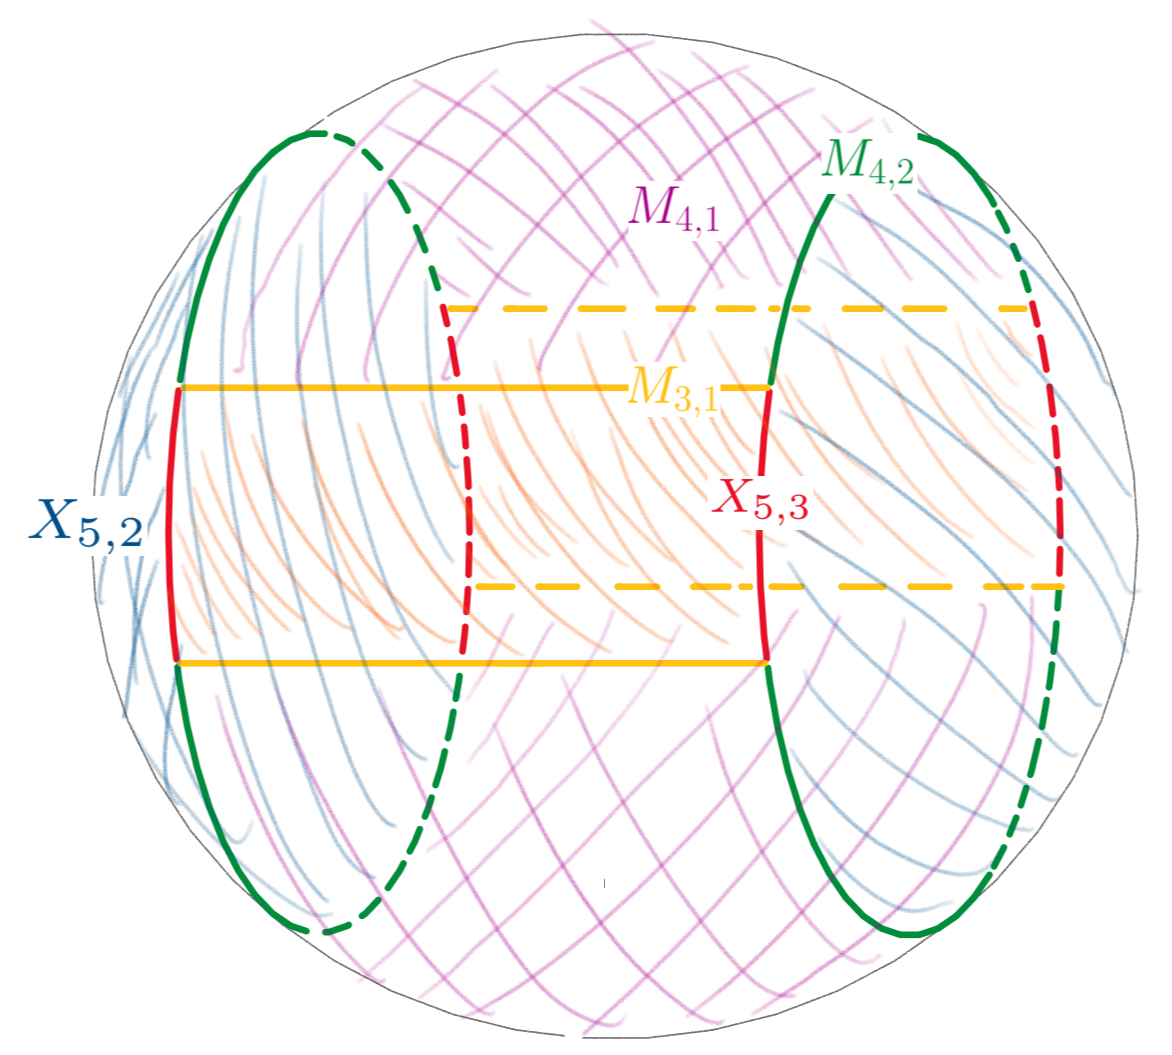
\includegraphics[width=\linewidth]{fig/differential.png}
      \captionof{figure}{
      We can see that $\colim D_{x_5}$ is a topological space that inherits a closed smooth manifolds structure.
      }
      \label{fig:test2}
    \end{minipage}
    \end{figure}
\end{exmp*}

\begin{restatable}{thmA}{ThA}\label{SSofStrFFCat}
    Let $\fC$ be a flow category with an $\cX$ tangential structure.
    There is a spectral sequence:
    \begin{equation*}
        \pg{E}{1}{n}{p} = \bigoplus_{\norm{z}=p} \Omega^{\cX}_{n-p}
    \end{equation*}
    which converges to the homotopy groups of the realization:
    \begin{equation*}
        \rnp{E} \implies \pi_n \norm{\fC}.
    \end{equation*}
    An element $X_z \in \pg{E}{1}{n}{p}$ survives to $\pg{E}{r+1}{n}{p}$ if and only if there is an $(X,r,n,p)$ extension of $\fC$. Let $\fC'$ be such an extension, the differential is represented geometrically by the Toda manifolds:
    \begin{equation*}
        d_{r+1}(X) = \bigsqcup_{y \in \fC_{p-(r+1)}} \colim D_y
    \end{equation*}
    viewed as an element
    \begin{equation*}
        d_{r+1}(X) \in \bigoplus_{y \in \fC_{p-(r+1)}} \Omega^{\cX}_{n-p+r} = \pg{E}{r+1}{n-1}{p-(r+1)}.
    \end{equation*}
\end{restatable}
We think of an existence of $(r,n,p)$-extension of $X$ as $X \in \ker\ d_r$.
\begin{rem}
    Different choice of framing
\end{rem}


A key tool used to prove \cref{SSofStrFFCat} is a description of the spectral sequence of a coherent chain complex in terms of chain complex maps.

\begin{restatable}{thmA}{ThB}\label{SSofCh}
    Let $K \in \Ch(\Sp)$ be a coherent chain complex in Spectra. Then we have a spectral sequence:
    \begin{equation*}
        E_1^{n,p} = \pi_{n - p} K_p,
    \end{equation*}
    which converges to
    \begin{equation*}
        E_r^{n,p} \implies \pi_n \colim_p (\cI K)_p,
    \end{equation*}
    
    Moreover, let $x: \mathbb{S}^{n - p} \to K_p$ represent an element in $\pg{E}{1}{n}{p}$. Then $x$ survives to $\pg{E}{r+1}{n}{p}$ if and only if there is a chain map:
    \begin{equation}\label{eq:x_ext}
        \xymatrix{
        \mathbb{S}^{n - p} \ar[d]_{x} \ar[r] & 0 \ar[r]\ar[d] & \dots \ar[r]\ar[d]& 0\ar[d]\\
        K_p \ar[r]^{d_p}& K_{p - 1} \ar[r]^{d_{p - 1}}& \dots \ar[r]^{d_{p - r + } \quad}& K_{p - r},
        }
    \end{equation}
    where the top row is concentrated in degree $p$, and the bottom row is the restriction of $K$.
    The differential $\partial_{r+1}(x)$ is given by the composition of chain maps:
    \begin{equation*}
        \xymatrix
        {   \mathbb{S}^{n-p} \ar[r]\ar[d]_x & \dots \ar[r]\ar[d] &  0 \ar[d]\\
            K_p \ar[r]\ar[d] & \dots \ar[r]\ar[d] &  K_{p-r} \ar[d] \\
            0 \ar[r] & \dots \ar[r] & K_{p-r-1} 
        }
    \end{equation*}
    where the first map is \cref{eq:x_ext} and the second is induced from the structure of the chain $K$.
\end{restatable}
We achieve this result by combining the description of the spectral sequence of a filtered object in Lurie's \cite{Lur17}, together with \cite{Ari21}.

\subsection*{Relation to other work}
This paper contributes to the broader project of providing a geometric model for Spectra. See \cite{abouzaid2024foundation} for the foundation of this project, which defines the stable $\infty$-category of framed flow categories and the equivalence to the category of Spectra.

This project traces back to CJS in \cite{CJS95}, who coined the term "flow category" as a way of organizing the data of a Morse-Smale function in a categorical way, constructing a coherent version of chain complexes from such a category and "realizing" these chains into a filtered spectrum. These ideas have proven to be very useful in Floer theory.

In knot theory, organizing the data of knots into a flow category results in a stable homotopy type that lifts Khovanov homology (see \cite{LS14}). After simplifying the flow categories (see \cite{lobb2018framed, lobb2017calculus}) and classifying 0 and 1 dimensional manifolds, they provide a combinatorial description and an effective algorithm to calculate the operations $\mathrm{Sq^2}: H^\ast(\fC, \mathbb{Z}/2) \to H^{\ast+2}(\fC, \mathbb{Z}/2)$ from a knot diagram, leading to the calculation of the homotopy (see \cite{lobb2020khovanov, lipshitz2014steenrod}). See \cite{marengon2024spectra} for a recap of flow categories in Khovanov and knot Floer theories.

This work is similar to our work in that we use the higher flow manifolds to calculate the differentials, which can be seen as higher cohomology operations.

In Hamiltonian Floer theory, one of the breakthroughs in the Arnold conjecture used a CJS-like construction—a generalization of flow categories suitable for the data of Hamiltonian flow—to prove a version of the Arnold conjecture over characteristic $p$ (see \cite{abouzaid2021arnold}). Similar ideas appeared in the integral Arnold conjecture (see \cite{rezchikov2022integral, bai2022arnold}).
Another recent development is Morse-Bott flow categories, which is the framework of flow categories where the function has critical sets (instead of isolated points) (see \cite{bonciocat2024revisiting}). Further development is putting an equivariant structure on such categories, which induces an equivariant structure on the realization spectrum, as a framework for cyclotomic methods in symplectic geometry (see \cite{cote2023equivariant, rezchikov2024cyclotomic}).

One can find flow-category-like constructions in Lagrangian geometry, which lifts the Fukaya category of a symplectic manifold (see \cite{porcelli2024bordism, porcelli2024spectral}).

\begin{rem}
    Note that in this paper we treat flow categories as chain complexes in $\Sp$ or filtered spectra. We expect that there is a similar construction to \cite{abouzaid2024foundation} that provides a flow-categorical model for $\{K_p\} \in \Ch(\Sp)$ such that $K_p = \bigoplus \mathbb{S}$.
\end{rem}

The interpretation of gluing manifolds as Toda brackets or Massey products appears in \cite{alexander1972cobordism}, where the author defines the Massey product as the gluing of two manifolds with boundary.

\cref{SSofCh} has a similar flavor to other works about spectral sequences associated with various objects. In \cite{Ari21}, the authors present the connection between filtered objects and coherent chain complexes and also define a spectral sequence of coherent chain complexes using the Beilinson t-structure. We also recommend \cite{antieau2024spectral} as an introduction to spectral sequences and the relation to chain complexes on one hand and to the spectral sequence of filtered objects defined in \cite{Lur17}.
The construction of the spectral sequence in this paper is similar to the papers \cite{blanc2022spectral}, where the authors define a spectral sequence of a simplicial object.

\subsection*{Paper layout}
Section 2 is dedicated to the framework of chain complexes in (stable) $\infty$ categories and the proof of \cref{SSofCh}.

In Section 3, we recall the definitions of manifolds with corners, framed flow categories, and the Pontryagin-Thom construction for manifolds with corners. At the end of the section, we show some properties of Pontryagin-Thom that will be useful in the following sections.

In Section 4, we construct a correspondence between chain complexes in the category of spectra (with values $\bigoplus \mathbb{S}$) and framed flow categories.

Our goal in the next two chapters is to upgrade this correspondence to play nicely with spectral sequences, in the sense that given a framed flow category, we can produce a spectral sequence of the corresponding chain complex and give a geometrical description of the pages and the differentials.

In Section 5, we compare different models for chain complexes through different models for infinity categories (topologically enriched, simplicially enriched, and simplicial sets). This allows us to give a simple description for the composition of maps of flow categories.

In Section 6, we translate the description of the composition of maps of flow categories into a geometrical description and claim the result of a spectral sequence of framed flow categories.

In the last section, we show how we can replace the framing structure with a general tangential structure and how different structures interact with each other. This section also contains examples of spectral sequences of flow categories.

\subsection*{Discussion and open problems}
\textbf{Different definitions for flow categories.} In \cite{abouzaid2024foundation} the authors construct an $\infty$-category $\mathrm{Flow^{\fr}}$ (see also \cite{porcelli2024bordism} for the homotopy category), and showed that it is equivalent to $\Sp$. We explain the main difference between our work and theirs from an algebro-topological point of view. Let $M$ be a compact manifold, we can take two Morse Smale functions, and get two framed flow categories, $\fC_f,\fC_g$, by interpolating between $f$ and $g$ we get two maps in $\mathrm{Flow^{\fr}}$
\begin{equation*}
    H_{f,g}: \fC_f \to \fC_g, \quad H_{g,f}: \fC_g \to \fC_f
\end{equation*}
and by homotoping the composition we get a 2-morphisms
\begin{equation*}
    H_{g,f} \circ H_{f,g} \simeq Id, \quad H_{f,g} \circ H_{g,f} \simeq Id.
\end{equation*}
Hence the flow category of $M$ independent of the choice of Morse Smale function.
On the other hand, $f$ and $g$ induces a CW structure on $M$, and different CW structures yield different (Atiyah–Hirzebruch) spectral sequences. So we can't define spectral sequence as invariant of the equivalence classes in $\mathrm{Flow^{\fr}}$.
To solve this problem, we believe that one can define another $\infty$ category, with different morphisms. For a 2 morphism $R$, between $\fC,\sD$, and two objects $x \in \fC, y \in \sD$ we ask that if $\norm{y} > \norm{x}$, then $R_{x,y} = \varnothing$ (instead of being $\norm{y}-\norm{x}$ manifold). This construction should result in a subcategory of $\Fil(\Sp)$ where the two Morse-Smale functions on a manifold $M$ give distinct objects.

In this paper the whole $\infty$-categorical structure It’s unnecessary and we define the equivalence relation on flow categories by pulling it back from the category $\Ch(\Sp)$ (see \cref{prop:FF_are_Ch}).
\subsection*{Acknowledgments}
\todo{Later}